\documentclass[1p]{elsarticle_modified}
%\bibliographystyle{elsarticle-num}

%\usepackage[colorlinks]{hyperref}
%\usepackage{abbrmath_seonhwa} %\Abb, \Ascr, \Acal ,\Abf, \Afrak
\usepackage{amsfonts}
\usepackage{amssymb}
\usepackage{amsmath}
\usepackage{amsthm}
\usepackage{scalefnt}
\usepackage{amsbsy}
\usepackage{kotex}
\usepackage{caption}
\usepackage{subfig}
\usepackage{color}
\usepackage{graphicx}
\usepackage{xcolor} %% white, black, red, green, blue, cyan, magenta, yellow
\usepackage{float}
\usepackage{setspace}
\usepackage{hyperref}

\usepackage{tikz}
\usetikzlibrary{arrows}

\usepackage{multirow}
\usepackage{array} % fixed length table
\usepackage{hhline}

%%%%%%%%%%%%%%%%%%%%%
\makeatletter
\renewcommand*\env@matrix[1][\arraystretch]{%
	\edef\arraystretch{#1}%
	\hskip -\arraycolsep
	\let\@ifnextchar\new@ifnextchar
	\array{*\c@MaxMatrixCols c}}
\makeatother %https://tex.stackexchange.com/questions/14071/how-can-i-increase-the-line-spacing-in-a-matrix
%%%%%%%%%%%%%%%

\usepackage[normalem]{ulem}

\newcommand{\msout}[1]{\ifmmode\text{\sout{\ensuremath{#1}}}\else\sout{#1}\fi}
%SOURCE: \msout is \stkout macro in https://tex.stackexchange.com/questions/20609/strikeout-in-math-mode

\newcommand{\cancel}[1]{
	\ifmmode
	{\color{red}\msout{#1}}
	\else
	{\color{red}\sout{#1}}
	\fi
}

\newcommand{\add}[1]{
	{\color{blue}\uwave{#1}}
}

\newcommand{\replace}[2]{
	\ifmmode
	{\color{red}\msout{#1}}{\color{blue}\uwave{#2}}
	\else
	{\color{red}\sout{#1}}{\color{blue}\uwave{#2}}
	\fi
}

\newcommand{\Sol}{\mathcal{S}} %segment
\newcommand{\D}{D} %diagram
\newcommand{\A}{\mathcal{A}} %arc


%%%%%%%%%%%%%%%%%%%%%%%%%%%%%5 test

\def\sl{\operatorname{\textup{SL}}(2,\Cbb)}
\def\psl{\operatorname{\textup{PSL}}(2,\Cbb)}
\def\quan{\mkern 1mu \triangleright \mkern 1mu}

\theoremstyle{definition}
\newtheorem{thm}{Theorem}[section]
\newtheorem{prop}[thm]{Proposition}
\newtheorem{lem}[thm]{Lemma}
\newtheorem{ques}[thm]{Question}
\newtheorem{cor}[thm]{Corollary}
\newtheorem{defn}[thm]{Definition}
\newtheorem{exam}[thm]{Example}
\newtheorem{rmk}[thm]{Remark}
\newtheorem{alg}[thm]{Algorithm}

\newcommand{\I}{\sqrt{-1}}
\begin{document}

%\begin{frontmatter}
%
%\title{Boundary parabolic representations of knots up to 8 crossings}
%
%%% Group authors per affiliation:
%\author{Yunhi Cho} 
%\address{Department of Mathematics, University of Seoul, Seoul, Korea}
%\ead{yhcho@uos.ac.kr}
%
%
%\author{Seonhwa Kim} %\fnref{s_kim}}
%\address{Center for Geometry and Physics, Institute for Basic Science, Pohang, 37673, Korea}
%\ead{ryeona17@ibs.re.kr}
%
%\author{Hyuk Kim}
%\address{Department of Mathematical Sciences, Seoul National University, Seoul 08826, Korea}
%\ead{hyukkim@snu.ac.kr}
%
%\author{Seokbeom Yoon}
%\address{Department of Mathematical Sciences, Seoul National University, Seoul, 08826,  Korea}
%\ead{sbyoon15@snu.ac.kr}
%
%\begin{abstract}
%We find all boundary parabolic representation of knots up to 8 crossings.
%
%\end{abstract}
%\begin{keyword}
%    \MSC[2010] 57M25 
%\end{keyword}
%
%\end{frontmatter}

%\linenumbers
%\tableofcontents
%
\newcommand\colored[1]{\textcolor{white}{\rule[-0.35ex]{0.8em}{1.4ex}}\kern-0.8em\color{red} #1}%
%\newcommand\colored[1]{\textcolor{white}{ #1}\kern-2.17ex	\textcolor{white}{ #1}\kern-1.81ex	\textcolor{white}{ #1}\kern-2.15ex\color{red}#1	}

{\Large $\underline{12n_{0441}~(K12n_{0441})}$}

\setlength{\tabcolsep}{10pt}
\renewcommand{\arraystretch}{1.6}
\vspace{1cm}\begin{tabular}{m{100pt}>{\centering\arraybackslash}m{274pt}}
\multirow{5}{120pt}{
	\centering
	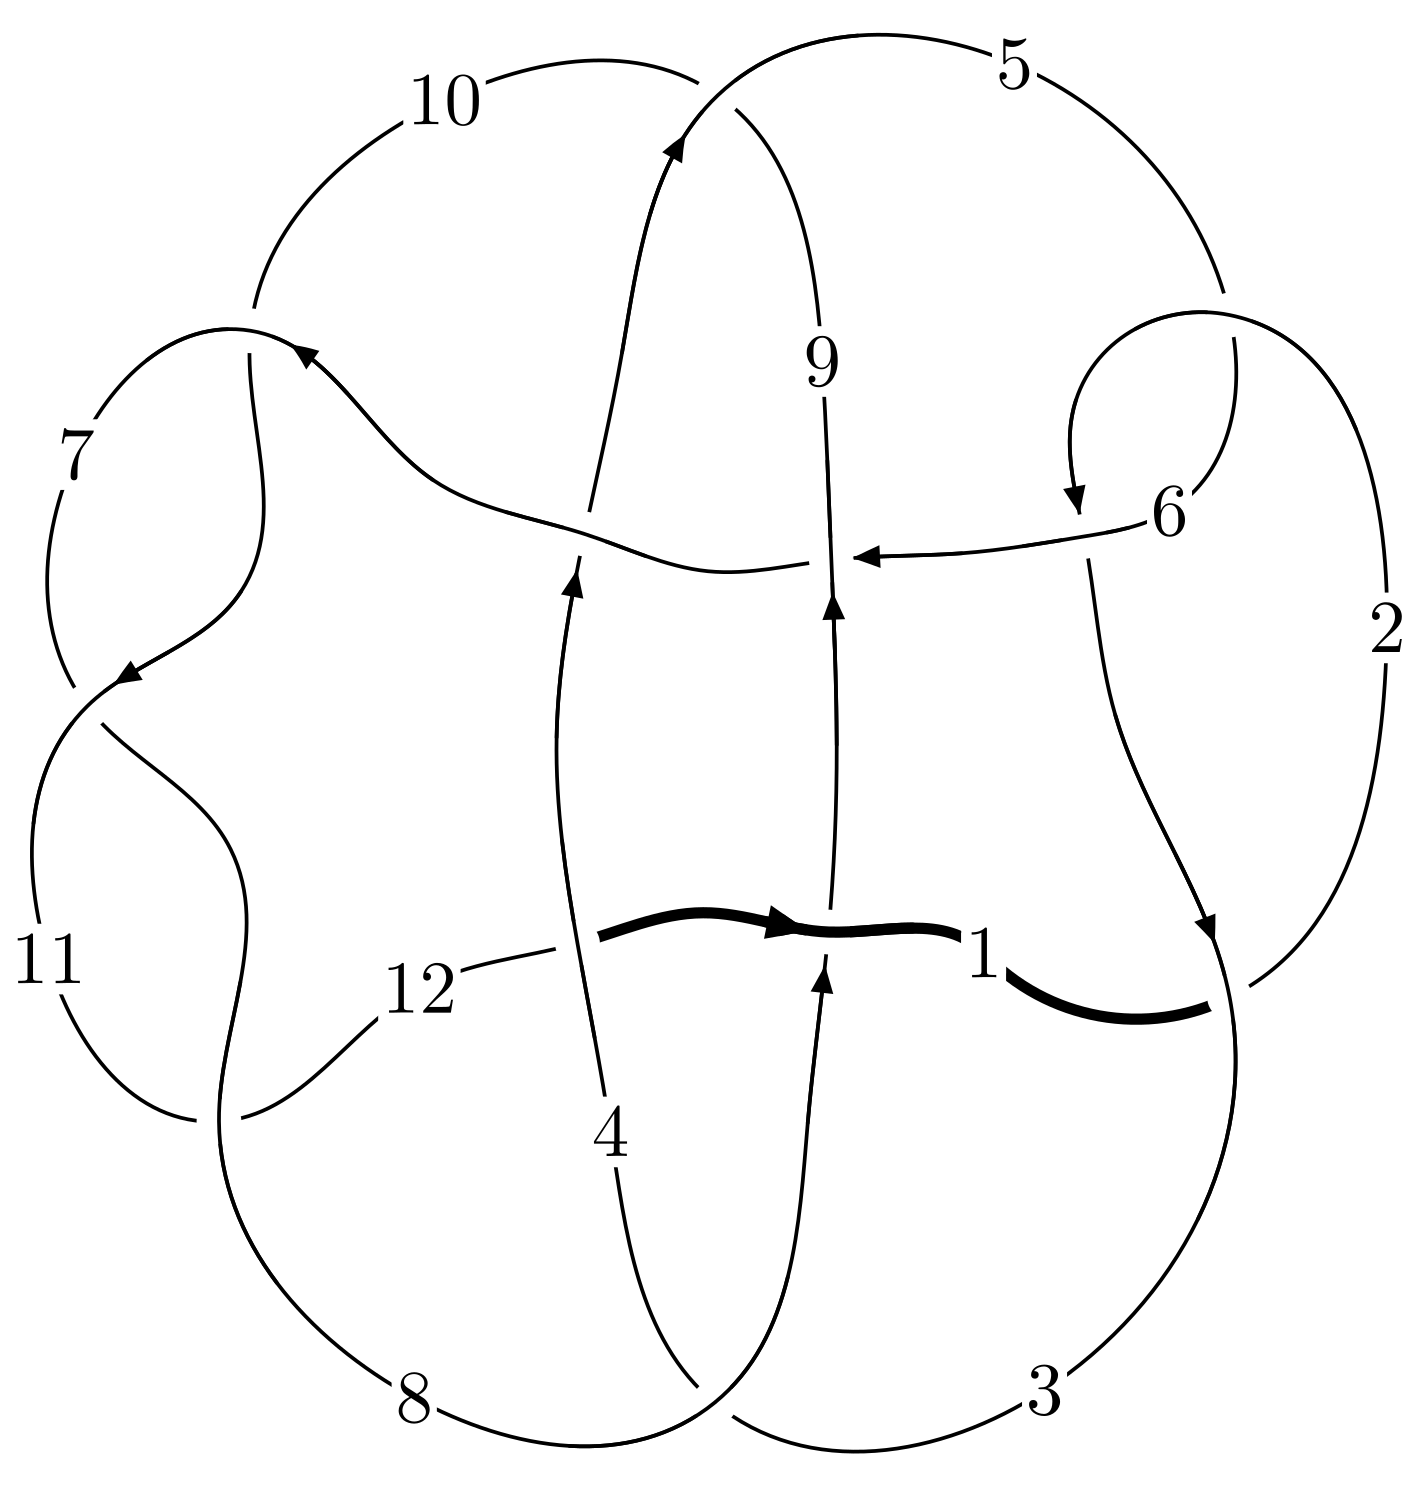
\includegraphics[width=112pt]{../../../GIT/diagram.site/Diagrams/png/2530_12n_0441.png}\\
\ \ \ A knot diagram\footnotemark}&
\allowdisplaybreaks
\textbf{Linearized knot diagam} \\
\cline{2-2}
 &
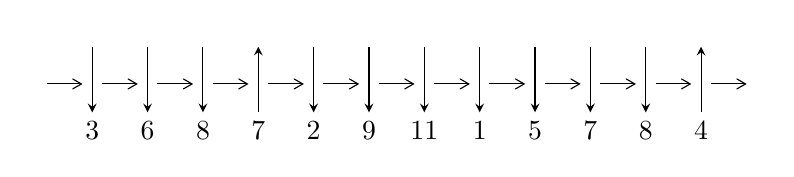
\begin{tikzpicture}[x=20pt, y=17pt]
	% nodes
	\node (C0) at (0, 0) {};
	\node (C1) at (1, 0) {};
	\node (C1U) at (1, +1) {};
	\node (C1D) at (1, -1) {3};

	\node (C2) at (2, 0) {};
	\node (C2U) at (2, +1) {};
	\node (C2D) at (2, -1) {6};

	\node (C3) at (3, 0) {};
	\node (C3U) at (3, +1) {};
	\node (C3D) at (3, -1) {8};

	\node (C4) at (4, 0) {};
	\node (C4U) at (4, +1) {};
	\node (C4D) at (4, -1) {7};

	\node (C5) at (5, 0) {};
	\node (C5U) at (5, +1) {};
	\node (C5D) at (5, -1) {2};

	\node (C6) at (6, 0) {};
	\node (C6U) at (6, +1) {};
	\node (C6D) at (6, -1) {9};

	\node (C7) at (7, 0) {};
	\node (C7U) at (7, +1) {};
	\node (C7D) at (7, -1) {11};

	\node (C8) at (8, 0) {};
	\node (C8U) at (8, +1) {};
	\node (C8D) at (8, -1) {1};

	\node (C9) at (9, 0) {};
	\node (C9U) at (9, +1) {};
	\node (C9D) at (9, -1) {5};

	\node (C10) at (10, 0) {};
	\node (C10U) at (10, +1) {};
	\node (C10D) at (10, -1) {7};

	\node (C11) at (11, 0) {};
	\node (C11U) at (11, +1) {};
	\node (C11D) at (11, -1) {8};

	\node (C12) at (12, 0) {};
	\node (C12U) at (12, +1) {};
	\node (C12D) at (12, -1) {4};
	\node (C13) at (13, 0) {};

	% arrows
	\draw[->,>={angle 60}]
	(C0) edge (C1) (C1) edge (C2) (C2) edge (C3) (C3) edge (C4) (C4) edge (C5) (C5) edge (C6) (C6) edge (C7) (C7) edge (C8) (C8) edge (C9) (C9) edge (C10) (C10) edge (C11) (C11) edge (C12) (C12) edge (C13) ;	\draw[->,>=stealth]
	(C1U) edge (C1D) (C2U) edge (C2D) (C3U) edge (C3D) (C4D) edge (C4U) (C5U) edge (C5D) (C6U) edge (C6D) (C7U) edge (C7D) (C8U) edge (C8D) (C9U) edge (C9D) (C10U) edge (C10D) (C11U) edge (C11D) (C12D) edge (C12U) ;
	\end{tikzpicture} \\
\hhline{~~} \\& 
\textbf{Solving Sequence} \\ \cline{2-2} 
 &
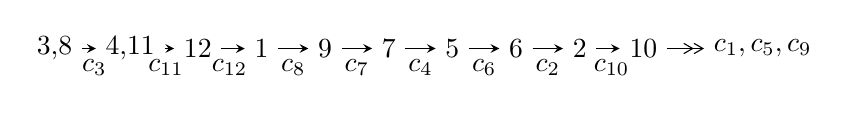
\begin{tikzpicture}[x=23pt, y=7pt]
	% node
	\node (A0) at (-1/8, 0) {3,8};
	\node (A1) at (17/16, 0) {4,11};
	\node (A2) at (17/8, 0) {12};
	\node (A3) at (25/8, 0) {1};
	\node (A4) at (33/8, 0) {9};
	\node (A5) at (41/8, 0) {7};
	\node (A6) at (49/8, 0) {5};
	\node (A7) at (57/8, 0) {6};
	\node (A8) at (65/8, 0) {2};
	\node (A9) at (73/8, 0) {10};
	\node (C1) at (1/2, -1) {$c_{3}$};
	\node (C2) at (13/8, -1) {$c_{11}$};
	\node (C3) at (21/8, -1) {$c_{12}$};
	\node (C4) at (29/8, -1) {$c_{8}$};
	\node (C5) at (37/8, -1) {$c_{7}$};
	\node (C6) at (45/8, -1) {$c_{4}$};
	\node (C7) at (53/8, -1) {$c_{6}$};
	\node (C8) at (61/8, -1) {$c_{2}$};
	\node (C9) at (69/8, -1) {$c_{10}$};
	\node (A10) at (11, 0) {$c_{1},c_{5},c_{9}$};

	% edge
	\draw[->,>=stealth]	
	(A0) edge (A1) (A1) edge (A2) (A2) edge (A3) (A3) edge (A4) (A4) edge (A5) (A5) edge (A6) (A6) edge (A7) (A7) edge (A8) (A8) edge (A9) ;
	\draw[->>,>={angle 60}]	
	(A9) edge (A10);
\end{tikzpicture} \\ 

\end{tabular} \\

\footnotetext{
The image of knot diagram is generated by the software ``\textbf{Draw programme}" developed by Andrew Bartholomew(\url{http://www.layer8.co.uk/maths/draw/index.htm\#Running-draw}), where we modified some parts for our purpose(\url{https://github.com/CATsTAILs/LinksPainter}).
}\phantom \\ \newline 
\centering \textbf{Ideals for irreducible components\footnotemark of $X_{\text{par}}$} 
 
\begin{align*}
I^u_{1}&=\langle 
-9309481822991 u^{25}+73829652568183 u^{24}+\cdots+260029930933511 b+103914726631843,\\
\phantom{I^u_{1}}&\phantom{= \langle  }469820212829242 u^{25}-103914726631843 u^{24}+\cdots+260029930933511 a+3878572919965900,\\
\phantom{I^u_{1}}&\phantom{= \langle  }u^{26}+11 u^{24}+\cdots+9 u+1\rangle \\
I^u_{2}&=\langle 
-2.76733\times10^{64} u^{39}-5.89505\times10^{64} u^{38}+\cdots+1.60944\times10^{63} b+2.15660\times10^{65},\\
\phantom{I^u_{2}}&\phantom{= \langle  }1.58706\times10^{65} u^{39}+3.38445\times10^{65} u^{38}+\cdots+1.60944\times10^{63} a-1.20443\times10^{66},\;u^{40}+2 u^{39}+\cdots-31 u+1\rangle \\
I^u_{3}&=\langle 
23 u^9+7 u^8+70 u^7+16 u^6+102 u^5+97 u^4+66 u^3+55 u^2+37 b-37 u-9,\\
\phantom{I^u_{3}}&\phantom{= \langle  }-56 u^9-9 u^8-201 u^7+27 u^6-369 u^5-56 u^4-402 u^3+72 u^2+37 a-37 u+149,\\
\phantom{I^u_{3}}&\phantom{= \langle  }u^{10}+4 u^8- u^7+8 u^6+9 u^4- u^3+2 u^2-2 u-1\rangle \\
I^u_{4}&=\langle 
-9 u^7+2 u^6-53 u^5+24 u^4-91 u^3+41 u^2+13 b-62 u+18,\\
\phantom{I^u_{4}}&\phantom{= \langle  }- u^7-6 u^5+2 u^4-10 u^3+6 u^2+a-7 u+4,\;u^8+6 u^6-2 u^5+10 u^4-6 u^3+7 u^2-4 u+1\rangle \\
I^u_{5}&=\langle 
b- u+1,\;a,\;u^2- u+1\rangle \\
\\
\end{align*}
\raggedright * 5 irreducible components of $\dim_{\mathbb{C}}=0$, with total 86 representations.\\
\footnotetext{All coefficients of polynomials are rational numbers. But the coefficients are sometimes approximated in decimal forms when there is not enough margin.}
\newpage
\renewcommand{\arraystretch}{1}
\centering \section*{I. $I^u_{1}= \langle -9.31\times10^{12} u^{25}+7.38\times10^{13} u^{24}+\cdots+2.60\times10^{14} b+1.04\times10^{14},\;4.70\times10^{14} u^{25}-1.04\times10^{14} u^{24}+\cdots+2.60\times10^{14} a+3.88\times10^{15},\;u^{26}+11 u^{24}+\cdots+9 u+1 \rangle$}
\flushleft \textbf{(i) Arc colorings}\\
\begin{tabular}{m{7pt} m{180pt} m{7pt} m{180pt} }
\flushright $a_{3}=$&$\begin{pmatrix}1\\0\end{pmatrix}$ \\
\flushright $a_{8}=$&$\begin{pmatrix}0\\u\end{pmatrix}$ \\
\flushright $a_{4}=$&$\begin{pmatrix}1\\u^2\end{pmatrix}$ \\
\flushright $a_{11}=$&$\begin{pmatrix}-1.80679 u^{25}+0.399626 u^{24}+\cdots-40.3048 u-14.9159\\0.0358016 u^{25}-0.283928 u^{24}+\cdots-0.789841 u-0.399626\end{pmatrix}$ \\
\flushright $a_{12}=$&$\begin{pmatrix}-1.80679 u^{25}+0.399626 u^{24}+\cdots-40.3048 u-14.9159\\0.0716032 u^{25}-0.567855 u^{24}+\cdots-2.57968 u-0.799252\end{pmatrix}$ \\
\flushright $a_{1}=$&$\begin{pmatrix}-1.77099 u^{25}+0.115699 u^{24}+\cdots-41.0946 u-15.3155\\-0.169902 u^{25}-0.371239 u^{24}+\cdots-0.0601367 u-0.515325\end{pmatrix}$ \\
\flushright $a_{9}=$&$\begin{pmatrix}3.57844 u^{25}-0.00928018 u^{24}+\cdots+60.7654 u+24.7620\\0.339222 u^{25}-0.587326 u^{24}+\cdots-7.69123 u-0.0242533\end{pmatrix}$ \\
\flushright $a_{7}=$&$\begin{pmatrix}-3.14858 u^{25}-0.276584 u^{24}+\cdots-69.8097 u-24.6725\\0.0250668 u^{25}+0.127352 u^{24}+\cdots+4.84799 u-0.123042\end{pmatrix}$ \\
\flushright $a_{5}=$&$\begin{pmatrix}0.0553456 u^{25}+0.301266 u^{24}+\cdots-9.68720 u-7.23255\\-0.0310923 u^{25}+0.0379551 u^{24}+\cdots-1.69626 u-0.240398\end{pmatrix}$ \\
\flushright $a_{6}=$&$\begin{pmatrix}1.98609 u^{25}-1.47838 u^{24}+\cdots+22.3075 u+16.0739\\-0.0620066 u^{25}+0.275777 u^{24}+\cdots+9.47790 u+1.77196\end{pmatrix}$ \\
\flushright $a_{2}=$&$\begin{pmatrix}-1.60109 u^{25}+0.486937 u^{24}+\cdots-41.0345 u-14.8002\\-0.169902 u^{25}-0.371239 u^{24}+\cdots-0.0601367 u-0.515325\end{pmatrix}$ \\
\flushright $a_{10}=$&$\begin{pmatrix}3.27718 u^{25}+0.178388 u^{24}+\cdots+68.4960 u+24.8174\\0.301266 u^{25}-0.187668 u^{24}+\cdots-7.73066 u-0.0553456\end{pmatrix}$\\&\end{tabular}
\flushleft \textbf{(ii) Obstruction class $= -1$}\\~\\
\flushleft \textbf{(iii) Cusp Shapes $= \frac{2458339353424590}{260029930933511} u^{25}+\frac{166778339040524}{260029930933511} u^{24}+\cdots+\frac{28387935709051593}{260029930933511} u+\frac{7983772528255336}{260029930933511}$}\\~\\
\newpage\renewcommand{\arraystretch}{1}
\flushleft \textbf{(iv) u-Polynomials at the component}\newline \\
\begin{tabular}{m{50pt}|m{274pt}}
Crossings & \hspace{64pt}u-Polynomials at each crossing \\
\hline $$\begin{aligned}c_{1}\end{aligned}$$&$\begin{aligned}
&u^{26}+7 u^{25}+\cdots+769 u+16
\end{aligned}$\\
\hline $$\begin{aligned}c_{2},c_{5}\end{aligned}$$&$\begin{aligned}
&u^{26}+7 u^{25}+\cdots-43 u-4
\end{aligned}$\\
\hline $$\begin{aligned}c_{3},c_{9}\end{aligned}$$&$\begin{aligned}
&u^{26}+11 u^{24}+\cdots+9 u+1
\end{aligned}$\\
\hline $$\begin{aligned}c_{4},c_{12}\end{aligned}$$&$\begin{aligned}
&u^{26}+2 u^{25}+\cdots+11 u+1
\end{aligned}$\\
\hline $$\begin{aligned}c_{6},c_{8}\end{aligned}$$&$\begin{aligned}
&u^{26}+u^{25}+\cdots- u-1
\end{aligned}$\\
\hline $$\begin{aligned}c_{7},c_{10},c_{11}\end{aligned}$$&$\begin{aligned}
&u^{26}+11 u^{25}+\cdots-23 u-2
\end{aligned}$\\
\hline
\end{tabular}\\~\\
\newpage\renewcommand{\arraystretch}{1}
\flushleft \textbf{(v) Riley Polynomials at the component}\newline \\
\begin{tabular}{m{50pt}|m{274pt}}
Crossings & \hspace{64pt}Riley Polynomials at each crossing \\
\hline $$\begin{aligned}c_{1}\end{aligned}$$&$\begin{aligned}
&y^{26}+17 y^{25}+\cdots-418017 y+256
\end{aligned}$\\
\hline $$\begin{aligned}c_{2},c_{5}\end{aligned}$$&$\begin{aligned}
&y^{26}-7 y^{25}+\cdots-769 y+16
\end{aligned}$\\
\hline $$\begin{aligned}c_{3},c_{9}\end{aligned}$$&$\begin{aligned}
&y^{26}+22 y^{25}+\cdots-33 y+1
\end{aligned}$\\
\hline $$\begin{aligned}c_{4},c_{12}\end{aligned}$$&$\begin{aligned}
&y^{26}-26 y^{25}+\cdots-17 y+1
\end{aligned}$\\
\hline $$\begin{aligned}c_{6},c_{8}\end{aligned}$$&$\begin{aligned}
&y^{26}-13 y^{25}+\cdots-5 y+1
\end{aligned}$\\
\hline $$\begin{aligned}c_{7},c_{10},c_{11}\end{aligned}$$&$\begin{aligned}
&y^{26}-3 y^{25}+\cdots-89 y+4
\end{aligned}$\\
\hline
\end{tabular}\\~\\
\newpage\flushleft \textbf{(vi) Complex Volumes and Cusp Shapes}
$$\begin{array}{c|c|c}  
\text{Solutions to }I^u_{1}& \I (\text{vol} + \sqrt{-1}CS) & \text{Cusp shape}\\
 \hline 
\begin{aligned}
u &= -0.925328 + 0.204781 I \\
a &= \phantom{-}0.576015 - 0.245577 I \\
b &= -0.549350 - 0.213489 I\end{aligned}
 & -1.185780 - 0.477506 I & -8.56678 - 2.27892 I \\ \hline\begin{aligned}
u &= -0.925328 - 0.204781 I \\
a &= \phantom{-}0.576015 + 0.245577 I \\
b &= -0.549350 + 0.213489 I\end{aligned}
 & -1.185780 + 0.477506 I & -8.56678 + 2.27892 I \\ \hline\begin{aligned}
u &= \phantom{-}0.437987 + 0.957320 I \\
a &= -1.273680 - 0.370591 I \\
b &= \phantom{-}1.67170 + 0.15777 I\end{aligned}
 & \phantom{-}4.40116 - 1.97219 I & -17.1827 - 0.9744 I \\ \hline\begin{aligned}
u &= \phantom{-}0.437987 - 0.957320 I \\
a &= -1.273680 + 0.370591 I \\
b &= \phantom{-}1.67170 - 0.15777 I\end{aligned}
 & \phantom{-}4.40116 + 1.97219 I & -17.1827 + 0.9744 I \\ \hline\begin{aligned}
u &= \phantom{-}0.248708 + 1.048740 I \\
a &= \phantom{-}0.062948 + 0.711511 I \\
b &= -0.187797 + 0.343031 I\end{aligned}
 & -1.73508 - 1.89801 I & -8.55455 + 3.04477 I \\ \hline\begin{aligned}
u &= \phantom{-}0.248708 - 1.048740 I \\
a &= \phantom{-}0.062948 - 0.711511 I \\
b &= -0.187797 - 0.343031 I\end{aligned}
 & -1.73508 + 1.89801 I & -8.55455 - 3.04477 I \\ \hline\begin{aligned}
u &= \phantom{-}1.033700 + 0.477780 I \\
a &= -0.441315 + 0.395879 I \\
b &= \phantom{-}0.271845 + 0.374508 I\end{aligned}
 & -1.59430 + 2.89984 I & -9.85116 - 8.11236 I \\ \hline\begin{aligned}
u &= \phantom{-}1.033700 - 0.477780 I \\
a &= -0.441315 - 0.395879 I \\
b &= \phantom{-}0.271845 - 0.374508 I\end{aligned}
 & -1.59430 - 2.89984 I & -9.85116 + 8.11236 I \\ \hline\begin{aligned}
u &= \phantom{-}0.152393 + 0.838106 I \\
a &= \phantom{-}0.304017 - 0.370147 I \\
b &= \phantom{-}0.040457 + 1.167170 I\end{aligned}
 & -1.68902 + 1.74396 I & -6.90590 - 3.41950 I \\ \hline\begin{aligned}
u &= \phantom{-}0.152393 - 0.838106 I \\
a &= \phantom{-}0.304017 + 0.370147 I \\
b &= \phantom{-}0.040457 - 1.167170 I\end{aligned}
 & -1.68902 - 1.74396 I & -6.90590 + 3.41950 I\\
 \hline 
 \end{array}$$\newpage$$\begin{array}{c|c|c}  
\text{Solutions to }I^u_{1}& \I (\text{vol} + \sqrt{-1}CS) & \text{Cusp shape}\\
 \hline 
\begin{aligned}
u &= \phantom{-}0.157882 + 1.174830 I \\
a &= \phantom{-}0.147312 + 0.389022 I \\
b &= -0.186083 + 0.702237 I\end{aligned}
 & -1.75577 - 1.91027 I & -7.85130 + 3.44778 I \\ \hline\begin{aligned}
u &= \phantom{-}0.157882 - 1.174830 I \\
a &= \phantom{-}0.147312 - 0.389022 I \\
b &= -0.186083 - 0.702237 I\end{aligned}
 & -1.75577 + 1.91027 I & -7.85130 - 3.44778 I \\ \hline\begin{aligned}
u &= -0.041568 + 1.314780 I \\
a &= -0.962386 + 0.969307 I \\
b &= \phantom{-}1.72636 - 0.25395 I\end{aligned}
 & \phantom{-}8.64541 + 0.35254 I & -5.05913 - 0.86290 I \\ \hline\begin{aligned}
u &= -0.041568 - 1.314780 I \\
a &= -0.962386 - 0.969307 I \\
b &= \phantom{-}1.72636 + 0.25395 I\end{aligned}
 & \phantom{-}8.64541 - 0.35254 I & -5.05913 + 0.86290 I \\ \hline\begin{aligned}
u &= \phantom{-}0.091023 + 1.338640 I \\
a &= \phantom{-}0.930924 + 0.895385 I \\
b &= -1.78763 - 0.03157 I\end{aligned}
 & \phantom{-}7.58539 - 7.09977 I & -6.01709 + 4.34352 I \\ \hline\begin{aligned}
u &= \phantom{-}0.091023 - 1.338640 I \\
a &= \phantom{-}0.930924 - 0.895385 I \\
b &= -1.78763 + 0.03157 I\end{aligned}
 & \phantom{-}7.58539 + 7.09977 I & -6.01709 - 4.34352 I \\ \hline\begin{aligned}
u &= -0.689089 + 1.219170 I \\
a &= \phantom{-}0.961669 + 0.093949 I \\
b &= -1.50398 - 0.49169 I\end{aligned}
 & -0.10698 + 7.65731 I & -11.70226 - 7.14009 I \\ \hline\begin{aligned}
u &= -0.689089 - 1.219170 I \\
a &= \phantom{-}0.961669 - 0.093949 I \\
b &= -1.50398 + 0.49169 I\end{aligned}
 & -0.10698 - 7.65731 I & -11.70226 + 7.14009 I \\ \hline\begin{aligned}
u &= -0.486762\phantom{ +0.000000I} \\
a &= \phantom{-}1.08934\phantom{ +0.000000I} \\
b &= -0.228656\phantom{ +0.000000I}\end{aligned}
 & -0.765965\phantom{ +0.000000I} & -12.9500\phantom{ +0.000000I} \\ \hline\begin{aligned}
u &= -0.098078 + 0.439549 I \\
a &= -0.77333 - 3.25861 I \\
b &= -0.237064 + 1.104460 I\end{aligned}
 & -5.10383 + 3.18903 I & -17.4273 - 3.2712 I\\
 \hline 
 \end{array}$$\newpage$$\begin{array}{c|c|c}  
\text{Solutions to }I^u_{1}& \I (\text{vol} + \sqrt{-1}CS) & \text{Cusp shape}\\
 \hline 
\begin{aligned}
u &= -0.098078 - 0.439549 I \\
a &= -0.77333 + 3.25861 I \\
b &= -0.237064 - 1.104460 I\end{aligned}
 & -5.10383 - 3.18903 I & -17.4273 + 3.2712 I \\ \hline\begin{aligned}
u &= \phantom{-}0.50591 + 1.51762 I \\
a &= -0.954886 + 0.422620 I \\
b &= \phantom{-}1.81183 - 0.81387 I\end{aligned}
 & \phantom{-}8.81872 - 9.45700 I & -5.57202 + 4.82775 I \\ \hline\begin{aligned}
u &= \phantom{-}0.50591 - 1.51762 I \\
a &= -0.954886 - 0.422620 I \\
b &= \phantom{-}1.81183 + 0.81387 I\end{aligned}
 & \phantom{-}8.81872 + 9.45700 I & -5.57202 - 4.82775 I \\ \hline\begin{aligned}
u &= -0.55589 + 1.59469 I \\
a &= \phantom{-}0.878916 + 0.428177 I \\
b &= -1.76028 - 0.92013 I\end{aligned}
 & \phantom{-}7.2466 + 15.9916 I & -8.00000 - 8.39864 I \\ \hline\begin{aligned}
u &= -0.55589 - 1.59469 I \\
a &= \phantom{-}0.878916 - 0.428177 I \\
b &= -1.76028 + 0.92013 I\end{aligned}
 & \phantom{-}7.2466 - 15.9916 I & -8.00000 + 8.39864 I \\ \hline\begin{aligned}
u &= -0.148557\phantom{ +0.000000I} \\
a &= -11.0018\phantom{ +0.000000I} \\
b &= -0.391355\phantom{ +0.000000I}\end{aligned}
 & -10.0986\phantom{ +0.000000I} & \phantom{-}22.3080\phantom{ +0.000000I}\\
 \hline 
 \end{array}$$\newpage\newpage\renewcommand{\arraystretch}{1}
\centering \section*{II. $I^u_{2}= \langle -2.77\times10^{64} u^{39}-5.90\times10^{64} u^{38}+\cdots+1.61\times10^{63} b+2.16\times10^{65},\;1.59\times10^{65} u^{39}+3.38\times10^{65} u^{38}+\cdots+1.61\times10^{63} a-1.20\times10^{66},\;u^{40}+2 u^{39}+\cdots-31 u+1 \rangle$}
\flushleft \textbf{(i) Arc colorings}\\
\begin{tabular}{m{7pt} m{180pt} m{7pt} m{180pt} }
\flushright $a_{3}=$&$\begin{pmatrix}1\\0\end{pmatrix}$ \\
\flushright $a_{8}=$&$\begin{pmatrix}0\\u\end{pmatrix}$ \\
\flushright $a_{4}=$&$\begin{pmatrix}1\\u^2\end{pmatrix}$ \\
\flushright $a_{11}=$&$\begin{pmatrix}-98.6099 u^{39}-210.287 u^{38}+\cdots-17327.2 u+748.357\\17.1944 u^{39}+36.6280 u^{38}+\cdots+3110.76 u-133.997\end{pmatrix}$ \\
\flushright $a_{12}=$&$\begin{pmatrix}-98.6099 u^{39}-210.287 u^{38}+\cdots-17327.2 u+748.357\\15.4838 u^{39}+32.9912 u^{38}+\cdots+2804.27 u-120.930\end{pmatrix}$ \\
\flushright $a_{1}=$&$\begin{pmatrix}-81.4155 u^{39}-173.659 u^{38}+\cdots-14216.5 u+614.359\\15.7727 u^{39}+33.5976 u^{38}+\cdots+2856.50 u-123.169\end{pmatrix}$ \\
\flushright $a_{9}=$&$\begin{pmatrix}24.3237 u^{39}+51.8494 u^{38}+\cdots+4186.11 u-167.565\\1.70809 u^{39}+3.60334 u^{38}+\cdots+350.584 u-14.1596\end{pmatrix}$ \\
\flushright $a_{7}=$&$\begin{pmatrix}-20.2827 u^{39}-43.3042 u^{38}+\cdots-3387.05 u+134.967\\-2.73705 u^{39}-5.80246 u^{38}+\cdots-523.421 u+21.6408\end{pmatrix}$ \\
\flushright $a_{5}=$&$\begin{pmatrix}13.0361 u^{39}+27.9037 u^{38}+\cdots+2358.25 u-112.609\\5.85766 u^{39}+12.5132 u^{38}+\cdots+1011.37 u-44.6712\end{pmatrix}$ \\
\flushright $a_{6}=$&$\begin{pmatrix}57.2063 u^{39}+121.962 u^{38}+\cdots+9989.28 u-428.196\\-12.1175 u^{39}-25.8205 u^{38}+\cdots-2184.36 u+94.7544\end{pmatrix}$ \\
\flushright $a_{2}=$&$\begin{pmatrix}-97.1883 u^{39}-207.257 u^{38}+\cdots-17073.0 u+737.528\\15.7727 u^{39}+33.5976 u^{38}+\cdots+2856.50 u-123.169\end{pmatrix}$ \\
\flushright $a_{10}=$&$\begin{pmatrix}-182.374 u^{39}-388.925 u^{38}+\cdots-32001.5 u+1381.43\\34.6744 u^{39}+73.8531 u^{38}+\cdots+6269.35 u-270.136\end{pmatrix}$\\&\end{tabular}
\flushleft \textbf{(ii) Obstruction class $= -1$}\\~\\
\flushleft \textbf{(iii) Cusp Shapes $= -21.2453 u^{39}-45.2764 u^{38}+\cdots-3927.04 u+165.006$}\\~\\
\newpage\renewcommand{\arraystretch}{1}
\flushleft \textbf{(iv) u-Polynomials at the component}\newline \\
\begin{tabular}{m{50pt}|m{274pt}}
Crossings & \hspace{64pt}u-Polynomials at each crossing \\
\hline $$\begin{aligned}c_{1}\end{aligned}$$&$\begin{aligned}
&(u^{20}+8 u^{19}+\cdots+67 u+9)^{2}
\end{aligned}$\\
\hline $$\begin{aligned}c_{2},c_{5}\end{aligned}$$&$\begin{aligned}
&(u^{20}-2 u^{19}+\cdots-7 u+3)^{2}
\end{aligned}$\\
\hline $$\begin{aligned}c_{3},c_{9}\end{aligned}$$&$\begin{aligned}
&u^{40}+2 u^{39}+\cdots-31 u+1
\end{aligned}$\\
\hline $$\begin{aligned}c_{4},c_{12}\end{aligned}$$&$\begin{aligned}
&u^{40}+4 u^{39}+\cdots+37 u+1
\end{aligned}$\\
\hline $$\begin{aligned}c_{6},c_{8}\end{aligned}$$&$\begin{aligned}
&u^{40}+u^{39}+\cdots-38 u+19
\end{aligned}$\\
\hline $$\begin{aligned}c_{7},c_{10},c_{11}\end{aligned}$$&$\begin{aligned}
&(u^{20}-5 u^{19}+\cdots-9 u+2)^{2}
\end{aligned}$\\
\hline
\end{tabular}\\~\\
\newpage\renewcommand{\arraystretch}{1}
\flushleft \textbf{(v) Riley Polynomials at the component}\newline \\
\begin{tabular}{m{50pt}|m{274pt}}
Crossings & \hspace{64pt}Riley Polynomials at each crossing \\
\hline $$\begin{aligned}c_{1}\end{aligned}$$&$\begin{aligned}
&(y^{20}+12 y^{19}+\cdots-223 y+81)^{2}
\end{aligned}$\\
\hline $$\begin{aligned}c_{2},c_{5}\end{aligned}$$&$\begin{aligned}
&(y^{20}-8 y^{19}+\cdots-67 y+9)^{2}
\end{aligned}$\\
\hline $$\begin{aligned}c_{3},c_{9}\end{aligned}$$&$\begin{aligned}
&y^{40}+40 y^{39}+\cdots+19 y+1
\end{aligned}$\\
\hline $$\begin{aligned}c_{4},c_{12}\end{aligned}$$&$\begin{aligned}
&y^{40}-36 y^{39}+\cdots-231 y+1
\end{aligned}$\\
\hline $$\begin{aligned}c_{6},c_{8}\end{aligned}$$&$\begin{aligned}
&y^{40}+y^{39}+\cdots+5548 y+361
\end{aligned}$\\
\hline $$\begin{aligned}c_{7},c_{10},c_{11}\end{aligned}$$&$\begin{aligned}
&(y^{20}- y^{19}+\cdots+15 y+4)^{2}
\end{aligned}$\\
\hline
\end{tabular}\\~\\
\newpage\flushleft \textbf{(vi) Complex Volumes and Cusp Shapes}
$$\begin{array}{c|c|c}  
\text{Solutions to }I^u_{2}& \I (\text{vol} + \sqrt{-1}CS) & \text{Cusp shape}\\
 \hline 
\begin{aligned}
u &= \phantom{-}0.107685 + 0.869000 I \\
a &= -0.09684 + 1.48156 I \\
b &= -0.316103 + 0.209805 I\end{aligned}
 & -1.93389 - 2.53032 I & -6.19592 + 4.02108 I \\ \hline\begin{aligned}
u &= \phantom{-}0.107685 - 0.869000 I \\
a &= -0.09684 - 1.48156 I \\
b &= -0.316103 - 0.209805 I\end{aligned}
 & -1.93389 + 2.53032 I & -6.19592 - 4.02108 I \\ \hline\begin{aligned}
u &= -0.373189 + 1.166640 I \\
a &= -0.636181 - 0.287370 I \\
b &= \phantom{-}1.69080 + 0.43538 I\end{aligned}
 & \phantom{-}2.80723 + 3.42080 I & \phantom{-0.000000 } 0 \\ \hline\begin{aligned}
u &= -0.373189 - 1.166640 I \\
a &= -0.636181 + 0.287370 I \\
b &= \phantom{-}1.69080 - 0.43538 I\end{aligned}
 & \phantom{-}2.80723 - 3.42080 I & \phantom{-0.000000 } 0 \\ \hline\begin{aligned}
u &= \phantom{-}1.163750 + 0.469682 I \\
a &= \phantom{-}0.612522 + 0.298397 I \\
b &= -0.004964 - 0.158740 I\end{aligned}
 & \phantom{-}2.80723 - 3.42080 I & \phantom{-0.000000 } 0 \\ \hline\begin{aligned}
u &= \phantom{-}1.163750 - 0.469682 I \\
a &= \phantom{-}0.612522 - 0.298397 I \\
b &= -0.004964 + 0.158740 I\end{aligned}
 & \phantom{-}2.80723 + 3.42080 I & \phantom{-0.000000 } 0 \\ \hline\begin{aligned}
u &= \phantom{-}0.091657 + 1.296970 I \\
a &= \phantom{-}0.932233 - 0.746341 I \\
b &= -1.73419 - 0.20045 I\end{aligned}
 & \phantom{-}8.52898 - 1.35152 I & \phantom{-0.000000 } 0 \\ \hline\begin{aligned}
u &= \phantom{-}0.091657 - 1.296970 I \\
a &= \phantom{-}0.932233 + 0.746341 I \\
b &= -1.73419 + 0.20045 I\end{aligned}
 & \phantom{-}8.52898 + 1.35152 I & \phantom{-0.000000 } 0 \\ \hline\begin{aligned}
u &= \phantom{-}0.231177 + 0.655143 I \\
a &= \phantom{-}0.791547 - 0.146798 I \\
b &= -1.64148 + 0.76911 I\end{aligned}
 & -2.77919 - 0.72470 I & -6.99365 + 10.58729 I \\ \hline\begin{aligned}
u &= \phantom{-}0.231177 - 0.655143 I \\
a &= \phantom{-}0.791547 + 0.146798 I \\
b &= -1.64148 - 0.76911 I\end{aligned}
 & -2.77919 + 0.72470 I & -6.99365 - 10.58729 I\\
 \hline 
 \end{array}$$\newpage$$\begin{array}{c|c|c}  
\text{Solutions to }I^u_{2}& \I (\text{vol} + \sqrt{-1}CS) & \text{Cusp shape}\\
 \hline 
\begin{aligned}
u &= \phantom{-}0.615112 + 1.163700 I \\
a &= \phantom{-}0.568955 - 0.258845 I \\
b &= -1.72547 + 0.43428 I\end{aligned}
 & \phantom{-}0.70919 - 8.81461 I & \phantom{-0.000000 } 0 \\ \hline\begin{aligned}
u &= \phantom{-}0.615112 - 1.163700 I \\
a &= \phantom{-}0.568955 + 0.258845 I \\
b &= -1.72547 - 0.43428 I\end{aligned}
 & \phantom{-}0.70919 + 8.81461 I & \phantom{-0.000000 } 0 \\ \hline\begin{aligned}
u &= -0.110827 + 1.329560 I \\
a &= \phantom{-}0.137120 + 0.964756 I \\
b &= \phantom{-}0.151293 - 0.864996 I\end{aligned}
 & -1.93389 - 2.53032 I & \phantom{-0.000000 } 0 \\ \hline\begin{aligned}
u &= -0.110827 - 1.329560 I \\
a &= \phantom{-}0.137120 - 0.964756 I \\
b &= \phantom{-}0.151293 + 0.864996 I\end{aligned}
 & -1.93389 + 2.53032 I & \phantom{-0.000000 } 0 \\ \hline\begin{aligned}
u &= \phantom{-}0.299939 + 1.358570 I \\
a &= -0.641788 - 0.218251 I \\
b &= \phantom{-}1.43525 - 0.13921 I\end{aligned}
 & \phantom{-}4.45736 - 0.35820 I & \phantom{-0.000000 } 0 \\ \hline\begin{aligned}
u &= \phantom{-}0.299939 - 1.358570 I \\
a &= -0.641788 + 0.218251 I \\
b &= \phantom{-}1.43525 + 0.13921 I\end{aligned}
 & \phantom{-}4.45736 + 0.35820 I & \phantom{-0.000000 } 0 \\ \hline\begin{aligned}
u &= -0.080772 + 1.395440 I \\
a &= -0.824582 - 0.752869 I \\
b &= \phantom{-}1.85230 - 0.03442 I\end{aligned}
 & \phantom{-}8.30234 + 6.78804 I & \phantom{-0.000000 } 0 \\ \hline\begin{aligned}
u &= -0.080772 - 1.395440 I \\
a &= -0.824582 + 0.752869 I \\
b &= \phantom{-}1.85230 + 0.03442 I\end{aligned}
 & \phantom{-}8.30234 - 6.78804 I & \phantom{-0.000000 } 0 \\ \hline\begin{aligned}
u &= \phantom{-}0.109439 + 0.536709 I \\
a &= \phantom{-}0.04901 + 1.66403 I \\
b &= -0.383758 + 1.251790 I\end{aligned}
 & -4.22584 + 1.07930 I & -18.8617 - 0.2582 I \\ \hline\begin{aligned}
u &= \phantom{-}0.109439 - 0.536709 I \\
a &= \phantom{-}0.04901 - 1.66403 I \\
b &= -0.383758 - 1.251790 I\end{aligned}
 & -4.22584 - 1.07930 I & -18.8617 + 0.2582 I\\
 \hline 
 \end{array}$$\newpage$$\begin{array}{c|c|c}  
\text{Solutions to }I^u_{2}& \I (\text{vol} + \sqrt{-1}CS) & \text{Cusp shape}\\
 \hline 
\begin{aligned}
u &= -1.38851 + 0.47418 I \\
a &= -0.073304 - 0.374070 I \\
b &= -0.386249 + 0.114590 I\end{aligned}
 & -2.77919 - 0.72470 I & \phantom{-0.000000 } 0 \\ \hline\begin{aligned}
u &= -1.38851 - 0.47418 I \\
a &= -0.073304 + 0.374070 I \\
b &= -0.386249 - 0.114590 I\end{aligned}
 & -2.77919 + 0.72470 I & \phantom{-0.000000 } 0 \\ \hline\begin{aligned}
u &= \phantom{-}0.48704 + 1.38580 I \\
a &= \phantom{-}0.839633 - 0.417130 I \\
b &= -1.128480 + 0.324249 I\end{aligned}
 & \phantom{-}4.71743 - 3.54403 I & \phantom{-0.000000 } 0 \\ \hline\begin{aligned}
u &= \phantom{-}0.48704 - 1.38580 I \\
a &= \phantom{-}0.839633 + 0.417130 I \\
b &= -1.128480 - 0.324249 I\end{aligned}
 & \phantom{-}4.71743 + 3.54403 I & \phantom{-0.000000 } 0 \\ \hline\begin{aligned}
u &= -0.40407 + 1.47756 I \\
a &= \phantom{-}0.618122 - 0.115570 I \\
b &= -1.342100 - 0.439927 I\end{aligned}
 & \phantom{-}3.26793 + 6.33523 I & \phantom{-0.000000 } 0 \\ \hline\begin{aligned}
u &= -0.40407 - 1.47756 I \\
a &= \phantom{-}0.618122 + 0.115570 I \\
b &= -1.342100 + 0.439927 I\end{aligned}
 & \phantom{-}3.26793 - 6.33523 I & \phantom{-0.000000 } 0 \\ \hline\begin{aligned}
u &= -0.27827 + 1.51128 I \\
a &= -0.730955 - 0.518496 I \\
b &= \phantom{-}1.66383 + 0.37308 I\end{aligned}
 & \phantom{-}4.71743 + 3.54403 I & \phantom{-0.000000 } 0 \\ \hline\begin{aligned}
u &= -0.27827 - 1.51128 I \\
a &= -0.730955 + 0.518496 I \\
b &= \phantom{-}1.66383 - 0.37308 I\end{aligned}
 & \phantom{-}4.71743 - 3.54403 I & \phantom{-0.000000 } 0 \\ \hline\begin{aligned}
u &= -1.54083 + 0.63283 I \\
a &= -0.476317 + 0.130739 I \\
b &= -0.0700266 + 0.0232375 I\end{aligned}
 & \phantom{-}0.70919 + 8.81461 I & \phantom{-0.000000 } 0 \\ \hline\begin{aligned}
u &= -1.54083 - 0.63283 I \\
a &= -0.476317 - 0.130739 I \\
b &= -0.0700266 - 0.0232375 I\end{aligned}
 & \phantom{-}0.70919 - 8.81461 I & \phantom{-0.000000 } 0\\
 \hline 
 \end{array}$$\newpage$$\begin{array}{c|c|c}  
\text{Solutions to }I^u_{2}& \I (\text{vol} + \sqrt{-1}CS) & \text{Cusp shape}\\
 \hline 
\begin{aligned}
u &= -0.35133 + 1.67126 I \\
a &= -0.780533 - 0.466237 I \\
b &= \phantom{-}1.62791 + 0.86433 I\end{aligned}
 & \phantom{-}8.52898 + 1.35152 I & \phantom{-0.000000 } 0 \\ \hline\begin{aligned}
u &= -0.35133 - 1.67126 I \\
a &= -0.780533 + 0.466237 I \\
b &= \phantom{-}1.62791 - 0.86433 I\end{aligned}
 & \phantom{-}8.52898 - 1.35152 I & \phantom{-0.000000 } 0 \\ \hline\begin{aligned}
u &= -0.17475 + 1.70544 I \\
a &= \phantom{-}0.173717 + 0.502733 I \\
b &= -0.090864 - 1.013700 I\end{aligned}
 & -4.22584 + 1.07930 I & \phantom{-0.000000 } 0 \\ \hline\begin{aligned}
u &= -0.17475 - 1.70544 I \\
a &= \phantom{-}0.173717 - 0.502733 I \\
b &= -0.090864 + 1.013700 I\end{aligned}
 & -4.22584 - 1.07930 I & \phantom{-0.000000 } 0 \\ \hline\begin{aligned}
u &= \phantom{-}0.42173 + 1.68142 I \\
a &= \phantom{-}0.766594 - 0.472156 I \\
b &= -1.44211 + 0.94264 I\end{aligned}
 & \phantom{-}8.30234 - 6.78804 I & \phantom{-0.000000 } 0 \\ \hline\begin{aligned}
u &= \phantom{-}0.42173 - 1.68142 I \\
a &= \phantom{-}0.766594 + 0.472156 I \\
b &= -1.44211 - 0.94264 I\end{aligned}
 & \phantom{-}8.30234 + 6.78804 I & \phantom{-0.000000 } 0 \\ \hline\begin{aligned}
u &= \phantom{-}0.1305640 + 0.0006413 I \\
a &= \phantom{-}0.76135 - 7.18315 I \\
b &= \phantom{-}0.314121 + 1.236250 I\end{aligned}
 & \phantom{-}4.45736 - 0.35820 I & -3.17120 - 1.48913 I \\ \hline\begin{aligned}
u &= \phantom{-}0.1305640 - 0.0006413 I \\
a &= \phantom{-}0.76135 + 7.18315 I \\
b &= \phantom{-}0.314121 - 1.236250 I\end{aligned}
 & \phantom{-}4.45736 + 0.35820 I & -3.17120 + 1.48913 I \\ \hline\begin{aligned}
u &= \phantom{-}0.0444473 + 0.0647209 I \\
a &= \phantom{-}9.50970 + 7.75152 I \\
b &= -0.46972 + 1.51512 I\end{aligned}
 & \phantom{-}3.26793 + 6.33523 I & -4.73548 - 4.55872 I \\ \hline\begin{aligned}
u &= \phantom{-}0.0444473 - 0.0647209 I \\
a &= \phantom{-}9.50970 - 7.75152 I \\
b &= -0.46972 - 1.51512 I\end{aligned}
 & \phantom{-}3.26793 - 6.33523 I & -4.73548 + 4.55872 I\\
 \hline 
 \end{array}$$\newpage\newpage\renewcommand{\arraystretch}{1}
\centering \section*{III. $I^u_{3}= \langle 23 u^9+7 u^8+\cdots+37 b-9,\;-56 u^9-9 u^8+\cdots+37 a+149,\;u^{10}+4 u^8- u^7+8 u^6+9 u^4- u^3+2 u^2-2 u-1 \rangle$}
\flushleft \textbf{(i) Arc colorings}\\
\begin{tabular}{m{7pt} m{180pt} m{7pt} m{180pt} }
\flushright $a_{3}=$&$\begin{pmatrix}1\\0\end{pmatrix}$ \\
\flushright $a_{8}=$&$\begin{pmatrix}0\\u\end{pmatrix}$ \\
\flushright $a_{4}=$&$\begin{pmatrix}1\\u^2\end{pmatrix}$ \\
\flushright $a_{11}=$&$\begin{pmatrix}\frac{56}{37} u^9+\frac{9}{37} u^8+\cdots+u-\frac{149}{37}\\-\frac{23}{37} u^9-\frac{7}{37} u^8+\cdots+u+\frac{9}{37}\end{pmatrix}$ \\
\flushright $a_{12}=$&$\begin{pmatrix}\frac{56}{37} u^9+\frac{9}{37} u^8+\cdots+u-\frac{149}{37}\\-1.24324 u^{9}-0.378378 u^{8}+\cdots+3 u+0.486486\end{pmatrix}$ \\
\flushright $a_{1}=$&$\begin{pmatrix}\frac{33}{37} u^9+\frac{2}{37} u^8+\cdots+2 u-\frac{140}{37}\\-0.648649 u^{9}-0.675676 u^{8}+\cdots+2 u+0.297297\end{pmatrix}$ \\
\flushright $a_{9}=$&$\begin{pmatrix}-1.89189 u^{9}-0.0540541 u^{8}+\cdots-5 u+5.78378\\\frac{1}{37} u^9+\frac{18}{37} u^8+\cdots-2 u-\frac{2}{37}\end{pmatrix}$ \\
\flushright $a_{7}=$&$\begin{pmatrix}2.21622 u^{9}+0.891892 u^{8}+\cdots+2 u-6.43243\\-0.324324 u^{9}-0.837838 u^{8}+\cdots+3 u+0.648649\end{pmatrix}$ \\
\flushright $a_{5}=$&$\begin{pmatrix}\frac{12}{37} u^9-\frac{6}{37} u^8+\cdots- u+\frac{87}{37}\\-\frac{10}{37} u^9+\frac{5}{37} u^8+\cdots- u-\frac{17}{37}\end{pmatrix}$ \\
\flushright $a_{6}=$&$\begin{pmatrix}-0.540541 u^{9}+1.27027 u^{8}+\cdots-6 u+3.08108\\-\frac{19}{37} u^9-\frac{9}{37} u^8+\cdots+u+\frac{38}{37}\end{pmatrix}$ \\
\flushright $a_{2}=$&$\begin{pmatrix}1.54054 u^{9}+0.729730 u^{8}+\cdots+0.162162 u^{2}-4.08108\\-0.648649 u^{9}-0.675676 u^{8}+\cdots+2 u+0.297297\end{pmatrix}$ \\
\flushright $a_{10}=$&$\begin{pmatrix}-2.05405 u^{9}-0.972973 u^{8}+\cdots-2 u+6.10811\\\frac{6}{37} u^9+\frac{34}{37} u^8+\cdots-3 u-\frac{12}{37}\end{pmatrix}$\\&\end{tabular}
\flushleft \textbf{(ii) Obstruction class $= 1$}\\~\\
\flushleft \textbf{(iii) Cusp Shapes $= \frac{205}{37} u^9-\frac{84}{37} u^8+\frac{936}{37} u^7-\frac{673}{37} u^6+\frac{2106}{37} u^5-\frac{1127}{37} u^4+\frac{2612}{37} u^3-\frac{1326}{37} u^2+23 u-\frac{1150}{37}$}\\~\\
\newpage\renewcommand{\arraystretch}{1}
\flushleft \textbf{(iv) u-Polynomials at the component}\newline \\
\begin{tabular}{m{50pt}|m{274pt}}
Crossings & \hspace{64pt}u-Polynomials at each crossing \\
\hline $$\begin{aligned}c_{1}\end{aligned}$$&$\begin{aligned}
&u^{10}-2 u^9+5 u^8-4 u^7+4 u^6-7 u^5+22 u^4-54 u^3+40 u^2-9 u+1
\end{aligned}$\\
\hline $$\begin{aligned}c_{2}\end{aligned}$$&$\begin{aligned}
&u^{10}+4 u^9+7 u^8+4 u^7-6 u^6-15 u^5-12 u^4+8 u^2+5 u+1
\end{aligned}$\\
\hline $$\begin{aligned}c_{3},c_{9}\end{aligned}$$&$\begin{aligned}
&u^{10}+4 u^8- u^7+8 u^6+9 u^4- u^3+2 u^2-2 u-1
\end{aligned}$\\
\hline $$\begin{aligned}c_{4},c_{12}\end{aligned}$$&$\begin{aligned}
&u^{10}+2 u^9-4 u^8-8 u^7+6 u^6+8 u^5-6 u^4+3 u^3+4 u^2-6 u+1
\end{aligned}$\\
\hline $$\begin{aligned}c_{5}\end{aligned}$$&$\begin{aligned}
&u^{10}-4 u^9+7 u^8-4 u^7-6 u^6+15 u^5-12 u^4+8 u^2-5 u+1
\end{aligned}$\\
\hline $$\begin{aligned}c_{6},c_{8}\end{aligned}$$&$\begin{aligned}
&u^{10}+u^9- u^8+2 u^7+u^6-2 u^5+3 u^4- u^3-2 u^2+2 u-1
\end{aligned}$\\
\hline $$\begin{aligned}c_{7}\end{aligned}$$&$\begin{aligned}
&u^{10}+8 u^9+\cdots-2 u-3
\end{aligned}$\\
\hline $$\begin{aligned}c_{10},c_{11}\end{aligned}$$&$\begin{aligned}
&u^{10}-8 u^9+\cdots+2 u-3
\end{aligned}$\\
\hline
\end{tabular}\\~\\
\newpage\renewcommand{\arraystretch}{1}
\flushleft \textbf{(v) Riley Polynomials at the component}\newline \\
\begin{tabular}{m{50pt}|m{274pt}}
Crossings & \hspace{64pt}Riley Polynomials at each crossing \\
\hline $$\begin{aligned}c_{1}\end{aligned}$$&$\begin{aligned}
&y^{10}+6 y^9+\cdots- y+1
\end{aligned}$\\
\hline $$\begin{aligned}c_{2},c_{5}\end{aligned}$$&$\begin{aligned}
&y^{10}-2 y^9+5 y^8-4 y^7+4 y^6-7 y^5+22 y^4-54 y^3+40 y^2-9 y+1
\end{aligned}$\\
\hline $$\begin{aligned}c_{3},c_{9}\end{aligned}$$&$\begin{aligned}
&y^{10}+8 y^9+\cdots-8 y+1
\end{aligned}$\\
\hline $$\begin{aligned}c_{4},c_{12}\end{aligned}$$&$\begin{aligned}
&y^{10}-12 y^9+\cdots-28 y+1
\end{aligned}$\\
\hline $$\begin{aligned}c_{6},c_{8}\end{aligned}$$&$\begin{aligned}
&y^{10}-3 y^9- y^8+4 y^7+y^6+4 y^5-5 y^4-7 y^3+2 y^2+1
\end{aligned}$\\
\hline $$\begin{aligned}c_{7},c_{10},c_{11}\end{aligned}$$&$\begin{aligned}
&y^{10}-6 y^9+5 y^8+13 y^7+47 y^5-51 y^4-237 y^3-174 y^2-88 y+9
\end{aligned}$\\
\hline
\end{tabular}\\~\\
\newpage\flushleft \textbf{(vi) Complex Volumes and Cusp Shapes}
$$\begin{array}{c|c|c}  
\text{Solutions to }I^u_{3}& \I (\text{vol} + \sqrt{-1}CS) & \text{Cusp shape}\\
 \hline 
\begin{aligned}
u &= -0.113601 + 0.927431 I \\
a &= -0.11490 - 1.98015 I \\
b &= -0.206295 + 0.774410 I\end{aligned}
 & -4.12954 + 3.49860 I & -9.01209 - 4.51290 I \\ \hline\begin{aligned}
u &= -0.113601 - 0.927431 I \\
a &= -0.11490 + 1.98015 I \\
b &= -0.206295 - 0.774410 I\end{aligned}
 & -4.12954 - 3.49860 I & -9.01209 + 4.51290 I \\ \hline\begin{aligned}
u &= -0.495456 + 0.987445 I \\
a &= -1.009770 + 0.387931 I \\
b &= \phantom{-}1.61173 - 0.28244 I\end{aligned}
 & \phantom{-}4.73376 + 2.16483 I & \phantom{-}1.22717 - 8.71022 I \\ \hline\begin{aligned}
u &= -0.495456 - 0.987445 I \\
a &= -1.009770 - 0.387931 I \\
b &= \phantom{-}1.61173 + 0.28244 I\end{aligned}
 & \phantom{-}4.73376 - 2.16483 I & \phantom{-}1.22717 + 8.71022 I \\ \hline\begin{aligned}
u &= \phantom{-}0.609357\phantom{ +0.000000I} \\
a &= -0.481071\phantom{ +0.000000I} \\
b &= -0.787987\phantom{ +0.000000I}\end{aligned}
 & -3.04786\phantom{ +0.000000I} & -13.9390\phantom{ +0.000000I} \\ \hline\begin{aligned}
u &= \phantom{-}0.84505 + 1.13903 I \\
a &= \phantom{-}0.589363 + 0.076741 I \\
b &= -1.336550 - 0.049223 I\end{aligned}
 & \phantom{-}2.04346 - 8.28564 I & -5.35537 + 8.10267 I \\ \hline\begin{aligned}
u &= \phantom{-}0.84505 - 1.13903 I \\
a &= \phantom{-}0.589363 - 0.076741 I \\
b &= -1.336550 + 0.049223 I\end{aligned}
 & \phantom{-}2.04346 + 8.28564 I & -5.35537 - 8.10267 I \\ \hline\begin{aligned}
u &= -0.37880 + 1.49046 I \\
a &= -0.751588 - 0.458927 I \\
b &= \phantom{-}1.42239 + 0.31186 I\end{aligned}
 & \phantom{-}5.62989 + 3.50299 I & -1.76700 - 2.21802 I \\ \hline\begin{aligned}
u &= -0.37880 - 1.49046 I \\
a &= -0.751588 + 0.458927 I \\
b &= \phantom{-}1.42239 - 0.31186 I\end{aligned}
 & \phantom{-}5.62989 - 3.50299 I & -1.76700 + 2.21802 I \\ \hline\begin{aligned}
u &= -0.323747\phantom{ +0.000000I} \\
a &= -4.94514\phantom{ +0.000000I} \\
b &= -0.194564\phantom{ +0.000000I}\end{aligned}
 & -10.2174\phantom{ +0.000000I} & -45.2470\phantom{ +0.000000I}\\
 \hline 
 \end{array}$$\newpage\newpage\renewcommand{\arraystretch}{1}
\centering \section*{IV. $I^u_{4}= \langle -9 u^7+2 u^6+\cdots+13 b+18,\;- u^7-6 u^5+2 u^4-10 u^3+6 u^2+a-7 u+4,\;u^8+6 u^6-2 u^5+10 u^4-6 u^3+7 u^2-4 u+1 \rangle$}
\flushleft \textbf{(i) Arc colorings}\\
\begin{tabular}{m{7pt} m{180pt} m{7pt} m{180pt} }
\flushright $a_{3}=$&$\begin{pmatrix}1\\0\end{pmatrix}$ \\
\flushright $a_{8}=$&$\begin{pmatrix}0\\u\end{pmatrix}$ \\
\flushright $a_{4}=$&$\begin{pmatrix}1\\u^2\end{pmatrix}$ \\
\flushright $a_{11}=$&$\begin{pmatrix}u^7+6 u^5-2 u^4+10 u^3-6 u^2+7 u-4\\0.692308 u^{7}-0.153846 u^{6}+\cdots+4.76923 u-1.38462\end{pmatrix}$ \\
\flushright $a_{12}=$&$\begin{pmatrix}u^7+6 u^5-2 u^4+10 u^3-6 u^2+7 u-4\\0.692308 u^{7}-0.153846 u^{6}+\cdots+3.76923 u-1.38462\end{pmatrix}$ \\
\flushright $a_{1}=$&$\begin{pmatrix}1.69231 u^{7}-0.153846 u^{6}+\cdots+11.7692 u-5.38462\\0.615385 u^{7}+0.307692 u^{6}+\cdots+2.46154 u-1.23077\end{pmatrix}$ \\
\flushright $a_{9}=$&$\begin{pmatrix}2.38462 u^{7}-0.307692 u^{6}+\cdots+17.5385 u-6.76923\\0.538462 u^{7}+0.769231 u^{6}+\cdots+3.15385 u-1.07692\end{pmatrix}$ \\
\flushright $a_{7}=$&$\begin{pmatrix}- u^7-6 u^5+2 u^4-10 u^3+6 u^2-7 u+4\\-0.692308 u^{7}+0.153846 u^{6}+\cdots-3.76923 u+1.38462\end{pmatrix}$ \\
\flushright $a_{5}=$&$\begin{pmatrix}1.38462 u^{7}+0.692308 u^{6}+\cdots+6.53846 u+0.230769\\-0.153846 u^{7}-0.0769231 u^{6}+\cdots+1.38462 u+0.307692\end{pmatrix}$ \\
\flushright $a_{6}=$&$\begin{pmatrix}-0.230769 u^{7}-0.615385 u^{6}+\cdots+1.07692 u+2.46154\\-0.846154 u^{7}+0.0769231 u^{6}+\cdots-3.38462 u+1.69231\end{pmatrix}$ \\
\flushright $a_{2}=$&$\begin{pmatrix}1.07692 u^{7}-0.461538 u^{6}+\cdots+9.30769 u-4.15385\\0.615385 u^{7}+0.307692 u^{6}+\cdots+2.46154 u-1.23077\end{pmatrix}$ \\
\flushright $a_{10}=$&$\begin{pmatrix}0\\u\end{pmatrix}$\\&\end{tabular}
\flushleft \textbf{(ii) Obstruction class $= 1$}\\~\\
\flushleft \textbf{(iii) Cusp Shapes $= -\frac{32}{13} u^7-\frac{16}{13} u^6-\frac{200}{13} u^5-\frac{36}{13} u^4-24 u^3+\frac{36}{13} u^2-\frac{128}{13} u-\frac{144}{13}$}\\~\\
\newpage\renewcommand{\arraystretch}{1}
\flushleft \textbf{(iv) u-Polynomials at the component}\newline \\
\begin{tabular}{m{50pt}|m{274pt}}
Crossings & \hspace{64pt}u-Polynomials at each crossing \\
\hline $$\begin{aligned}c_{1}\end{aligned}$$&$\begin{aligned}
&(u^2- u+1)^4
\end{aligned}$\\
\hline $$\begin{aligned}c_{2},c_{5}\end{aligned}$$&$\begin{aligned}
&(u^4- u^2+1)^2
\end{aligned}$\\
\hline $$\begin{aligned}c_{3},c_{9}\end{aligned}$$&$\begin{aligned}
&u^8+6 u^6-2 u^5+10 u^4-6 u^3+7 u^2-4 u+1
\end{aligned}$\\
\hline $$\begin{aligned}c_{4},c_{12}\end{aligned}$$&$\begin{aligned}
&(u^2+1)^4
\end{aligned}$\\
\hline $$\begin{aligned}c_{6},c_{8}\end{aligned}$$&$\begin{aligned}
&u^8-4 u^7+2 u^6+8 u^5-6 u^4-6 u^3+3 u^2+2 u+1
\end{aligned}$\\
\hline $$\begin{aligned}c_{7}\end{aligned}$$&$\begin{aligned}
&(u-1)^8
\end{aligned}$\\
\hline $$\begin{aligned}c_{10},c_{11}\end{aligned}$$&$\begin{aligned}
&(u+1)^8
\end{aligned}$\\
\hline
\end{tabular}\\~\\
\newpage\renewcommand{\arraystretch}{1}
\flushleft \textbf{(v) Riley Polynomials at the component}\newline \\
\begin{tabular}{m{50pt}|m{274pt}}
Crossings & \hspace{64pt}Riley Polynomials at each crossing \\
\hline $$\begin{aligned}c_{1}\end{aligned}$$&$\begin{aligned}
&(y^2+y+1)^4
\end{aligned}$\\
\hline $$\begin{aligned}c_{2},c_{5}\end{aligned}$$&$\begin{aligned}
&(y^2- y+1)^4
\end{aligned}$\\
\hline $$\begin{aligned}c_{3},c_{9}\end{aligned}$$&$\begin{aligned}
&y^8+12 y^7+56 y^6+130 y^5+162 y^4+100 y^3+21 y^2-2 y+1
\end{aligned}$\\
\hline $$\begin{aligned}c_{4},c_{12}\end{aligned}$$&$\begin{aligned}
&(y+1)^8
\end{aligned}$\\
\hline $$\begin{aligned}c_{6},c_{8}\end{aligned}$$&$\begin{aligned}
&y^8-12 y^7+56 y^6-130 y^5+162 y^4-100 y^3+21 y^2+2 y+1
\end{aligned}$\\
\hline $$\begin{aligned}c_{7},c_{10},c_{11}\end{aligned}$$&$\begin{aligned}
&(y-1)^8
\end{aligned}$\\
\hline
\end{tabular}\\~\\
\newpage\flushleft \textbf{(vi) Complex Volumes and Cusp Shapes}
$$\begin{array}{c|c|c}  
\text{Solutions to }I^u_{4}& \I (\text{vol} + \sqrt{-1}CS) & \text{Cusp shape}\\
 \hline 
\begin{aligned}
u &= \phantom{-}0.170691 + 0.964637 I \\
a &= -0.177866 + 1.005190 I \\
b &= \phantom{-0.000000 -}1.000000 I\end{aligned}
 & -3.28987 - 2.02988 I & -14.0000 + 3.4641 I \\ \hline\begin{aligned}
u &= \phantom{-}0.170691 - 0.964637 I \\
a &= -0.177866 - 1.005190 I \\
b &= \phantom{-0.000000 } -1.000000 I\end{aligned}
 & -3.28987 + 2.02988 I & -14.0000 - 3.4641 I \\ \hline\begin{aligned}
u &= -0.351035 + 1.212180 I \\
a &= \phantom{-}0.220415 + 0.761130 I \\
b &= \phantom{-0.000000 } -1.000000 I\end{aligned}
 & -3.28987 - 2.02988 I & -14.0000 + 3.4641 I \\ \hline\begin{aligned}
u &= -0.351035 - 1.212180 I \\
a &= \phantom{-}0.220415 - 0.761130 I \\
b &= \phantom{-0.000000 -}1.000000 I\end{aligned}
 & -3.28987 + 2.02988 I & -14.0000 - 3.4641 I \\ \hline\begin{aligned}
u &= \phantom{-}0.351035 + 0.212180 I \\
a &= -2.08644 + 1.26113 I \\
b &= \phantom{-0.000000 -}1.000000 I\end{aligned}
 & -3.28987 + 2.02988 I & -14.0000 - 3.4641 I \\ \hline\begin{aligned}
u &= \phantom{-}0.351035 - 0.212180 I \\
a &= -2.08644 - 1.26113 I \\
b &= \phantom{-0.000000 } -1.000000 I\end{aligned}
 & -3.28987 - 2.02988 I & -14.0000 + 3.4641 I \\ \hline\begin{aligned}
u &= -0.17069 + 1.96464 I \\
a &= \phantom{-}0.043891 + 0.505187 I \\
b &= \phantom{-0.000000 } -1.000000 I\end{aligned}
 & -3.28987 + 2.02988 I & -14.0000 - 3.4641 I \\ \hline\begin{aligned}
u &= -0.17069 - 1.96464 I \\
a &= \phantom{-}0.043891 - 0.505187 I \\
b &= \phantom{-0.000000 -}1.000000 I\end{aligned}
 & -3.28987 - 2.02988 I & -14.0000 + 3.4641 I\\
 \hline 
 \end{array}$$\newpage\newpage\renewcommand{\arraystretch}{1}
\centering \section*{V. $I^u_{5}= \langle b- u+1,\;a,\;u^2- u+1 \rangle$}
\flushleft \textbf{(i) Arc colorings}\\
\begin{tabular}{m{7pt} m{180pt} m{7pt} m{180pt} }
\flushright $a_{3}=$&$\begin{pmatrix}1\\0\end{pmatrix}$ \\
\flushright $a_{8}=$&$\begin{pmatrix}0\\u\end{pmatrix}$ \\
\flushright $a_{4}=$&$\begin{pmatrix}1\\u-1\end{pmatrix}$ \\
\flushright $a_{11}=$&$\begin{pmatrix}0\\u-1\end{pmatrix}$ \\
\flushright $a_{12}=$&$\begin{pmatrix}0\\u-1\end{pmatrix}$ \\
\flushright $a_{1}=$&$\begin{pmatrix}u-1\\-1\end{pmatrix}$ \\
\flushright $a_{9}=$&$\begin{pmatrix}u-1\\u-1\end{pmatrix}$ \\
\flushright $a_{7}=$&$\begin{pmatrix}0\\u\end{pmatrix}$ \\
\flushright $a_{5}=$&$\begin{pmatrix}1\\0\end{pmatrix}$ \\
\flushright $a_{6}=$&$\begin{pmatrix}- u+1\\1\end{pmatrix}$ \\
\flushright $a_{2}=$&$\begin{pmatrix}u\\-1\end{pmatrix}$ \\
\flushright $a_{10}=$&$\begin{pmatrix}0\\u-1\end{pmatrix}$\\&\end{tabular}
\flushleft \textbf{(ii) Obstruction class $= 1$}\\~\\
\flushleft \textbf{(iii) Cusp Shapes $= -15$}\\~\\
\newpage\renewcommand{\arraystretch}{1}
\flushleft \textbf{(iv) u-Polynomials at the component}\newline \\
\begin{tabular}{m{50pt}|m{274pt}}
Crossings & \hspace{64pt}u-Polynomials at each crossing \\
\hline $$\begin{aligned}c_{1},c_{2},c_{6}\\c_{8}\end{aligned}$$&$\begin{aligned}
&(u-1)^2
\end{aligned}$\\
\hline $$\begin{aligned}c_{3},c_{4},c_{9}\\c_{12}\end{aligned}$$&$\begin{aligned}
&u^2- u+1
\end{aligned}$\\
\hline $$\begin{aligned}c_{5}\end{aligned}$$&$\begin{aligned}
&(u+1)^2
\end{aligned}$\\
\hline $$\begin{aligned}c_{7},c_{10},c_{11}\end{aligned}$$&$\begin{aligned}
&u^2
\end{aligned}$\\
\hline
\end{tabular}\\~\\
\newpage\renewcommand{\arraystretch}{1}
\flushleft \textbf{(v) Riley Polynomials at the component}\newline \\
\begin{tabular}{m{50pt}|m{274pt}}
Crossings & \hspace{64pt}Riley Polynomials at each crossing \\
\hline $$\begin{aligned}c_{1},c_{2},c_{5}\\c_{6},c_{8}\end{aligned}$$&$\begin{aligned}
&(y-1)^2
\end{aligned}$\\
\hline $$\begin{aligned}c_{3},c_{4},c_{9}\\c_{12}\end{aligned}$$&$\begin{aligned}
&y^2+y+1
\end{aligned}$\\
\hline $$\begin{aligned}c_{7},c_{10},c_{11}\end{aligned}$$&$\begin{aligned}
&y^2
\end{aligned}$\\
\hline
\end{tabular}\\~\\
\newpage\flushleft \textbf{(vi) Complex Volumes and Cusp Shapes}
$$\begin{array}{c|c|c}  
\text{Solutions to }I^u_{5}& \I (\text{vol} + \sqrt{-1}CS) & \text{Cusp shape}\\
 \hline 
\begin{aligned}
u &= \phantom{-}0.500000 + 0.866025 I \\
a &= \phantom{-0.000000 } 0 \\
b &= -0.500000 + 0.866025 I\end{aligned}
 & -3.28987\phantom{ +0.000000I} & -15.0000\phantom{ +0.000000I} \\ \hline\begin{aligned}
u &= \phantom{-}0.500000 - 0.866025 I \\
a &= \phantom{-0.000000 } 0 \\
b &= -0.500000 - 0.866025 I\end{aligned}
 & -3.28987\phantom{ +0.000000I} & -15.0000\phantom{ +0.000000I}\\
 \hline 
 \end{array}$$\newpage
\newpage\renewcommand{\arraystretch}{1}
\centering \section*{ VI. u-Polynomials}
\begin{tabular}{m{50pt}|m{274pt}}
Crossings & \hspace{64pt}u-Polynomials at each crossing \\
\hline $$\begin{aligned}c_{1}\end{aligned}$$&$\begin{aligned}
&(u-1)^2(u^2- u+1)^4\\
&\cdot(u^{10}-2 u^9+5 u^8-4 u^7+4 u^6-7 u^5+22 u^4-54 u^3+40 u^2-9 u+1)\\
&\cdot((u^{20}+8 u^{19}+\cdots+67 u+9)^{2})(u^{26}+7 u^{25}+\cdots+769 u+16)
\end{aligned}$\\
\hline $$\begin{aligned}c_{2}\end{aligned}$$&$\begin{aligned}
&(u-1)^2(u^4- u^2+1)^2\\
&\cdot(u^{10}+4 u^9+7 u^8+4 u^7-6 u^6-15 u^5-12 u^4+8 u^2+5 u+1)\\
&\cdot((u^{20}-2 u^{19}+\cdots-7 u+3)^{2})(u^{26}+7 u^{25}+\cdots-43 u-4)
\end{aligned}$\\
\hline $$\begin{aligned}c_{3},c_{9}\end{aligned}$$&$\begin{aligned}
&(u^2- u+1)(u^8+6 u^6-2 u^5+10 u^4-6 u^3+7 u^2-4 u+1)\\
&\cdot(u^{10}+4 u^8- u^7+8 u^6+9 u^4- u^3+2 u^2-2 u-1)\\
&\cdot(u^{26}+11 u^{24}+\cdots+9 u+1)(u^{40}+2 u^{39}+\cdots-31 u+1)
\end{aligned}$\\
\hline $$\begin{aligned}c_{4},c_{12}\end{aligned}$$&$\begin{aligned}
&(u^2+1)^4(u^2- u+1)\\
&\cdot(u^{10}+2 u^9-4 u^8-8 u^7+6 u^6+8 u^5-6 u^4+3 u^3+4 u^2-6 u+1)\\
&\cdot(u^{26}+2 u^{25}+\cdots+11 u+1)(u^{40}+4 u^{39}+\cdots+37 u+1)
\end{aligned}$\\
\hline $$\begin{aligned}c_{5}\end{aligned}$$&$\begin{aligned}
&(u+1)^2(u^4- u^2+1)^2\\
&\cdot(u^{10}-4 u^9+7 u^8-4 u^7-6 u^6+15 u^5-12 u^4+8 u^2-5 u+1)\\
&\cdot((u^{20}-2 u^{19}+\cdots-7 u+3)^{2})(u^{26}+7 u^{25}+\cdots-43 u-4)
\end{aligned}$\\
\hline $$\begin{aligned}c_{6},c_{8}\end{aligned}$$&$\begin{aligned}
&(u-1)^2(u^8-4 u^7+2 u^6+8 u^5-6 u^4-6 u^3+3 u^2+2 u+1)\\
&\cdot(u^{10}+u^9- u^8+2 u^7+u^6-2 u^5+3 u^4- u^3-2 u^2+2 u-1)\\
&\cdot(u^{26}+u^{25}+\cdots- u-1)(u^{40}+u^{39}+\cdots-38 u+19)
\end{aligned}$\\
\hline $$\begin{aligned}c_{7}\end{aligned}$$&$\begin{aligned}
&u^2(u-1)^8(u^{10}+8 u^{9}+\cdots-2 u-3)(u^{20}-5 u^{19}+\cdots-9 u+2)^{2}\\
&\cdot(u^{26}+11 u^{25}+\cdots-23 u-2)
\end{aligned}$\\
\hline $$\begin{aligned}c_{10},c_{11}\end{aligned}$$&$\begin{aligned}
&u^2(u+1)^8(u^{10}-8 u^{9}+\cdots+2 u-3)(u^{20}-5 u^{19}+\cdots-9 u+2)^{2}\\
&\cdot(u^{26}+11 u^{25}+\cdots-23 u-2)
\end{aligned}$\\
\hline
\end{tabular}\newpage\renewcommand{\arraystretch}{1}
\centering \section*{ VII. Riley Polynomials}
\begin{tabular}{m{50pt}|m{274pt}}
Crossings & \hspace{64pt}Riley Polynomials at each crossing \\
\hline $$\begin{aligned}c_{1}\end{aligned}$$&$\begin{aligned}
&((y-1)^2)(y^2+y+1)^4(y^{10}+6 y^9+\cdots- y+1)\\
&\cdot(y^{20}+12 y^{19}+\cdots-223 y+81)^{2}\\
&\cdot(y^{26}+17 y^{25}+\cdots-418017 y+256)
\end{aligned}$\\
\hline $$\begin{aligned}c_{2},c_{5}\end{aligned}$$&$\begin{aligned}
&(y-1)^2(y^2- y+1)^4\\
&\cdot(y^{10}-2 y^9+5 y^8-4 y^7+4 y^6-7 y^5+22 y^4-54 y^3+40 y^2-9 y+1)\\
&\cdot((y^{20}-8 y^{19}+\cdots-67 y+9)^{2})(y^{26}-7 y^{25}+\cdots-769 y+16)
\end{aligned}$\\
\hline $$\begin{aligned}c_{3},c_{9}\end{aligned}$$&$\begin{aligned}
&(y^2+y+1)\\
&\cdot(y^8+12 y^7+56 y^6+130 y^5+162 y^4+100 y^3+21 y^2-2 y+1)\\
&\cdot(y^{10}+8 y^9+\cdots-8 y+1)(y^{26}+22 y^{25}+\cdots-33 y+1)\\
&\cdot(y^{40}+40 y^{39}+\cdots+19 y+1)
\end{aligned}$\\
\hline $$\begin{aligned}c_{4},c_{12}\end{aligned}$$&$\begin{aligned}
&((y+1)^8)(y^2+y+1)(y^{10}-12 y^9+\cdots-28 y+1)\\
&\cdot(y^{26}-26 y^{25}+\cdots-17 y+1)(y^{40}-36 y^{39}+\cdots-231 y+1)
\end{aligned}$\\
\hline $$\begin{aligned}c_{6},c_{8}\end{aligned}$$&$\begin{aligned}
&((y-1)^2)(y^8-12 y^7+\cdots+2 y+1)\\
&\cdot(y^{10}-3 y^9- y^8+4 y^7+y^6+4 y^5-5 y^4-7 y^3+2 y^2+1)\\
&\cdot(y^{26}-13 y^{25}+\cdots-5 y+1)(y^{40}+y^{39}+\cdots+5548 y+361)
\end{aligned}$\\
\hline $$\begin{aligned}c_{7},c_{10},c_{11}\end{aligned}$$&$\begin{aligned}
&y^2(y-1)^8\\
&\cdot(y^{10}-6 y^9+5 y^8+13 y^7+47 y^5-51 y^4-237 y^3-174 y^2-88 y+9)\\
&\cdot((y^{20}- y^{19}+\cdots+15 y+4)^{2})(y^{26}-3 y^{25}+\cdots-89 y+4)
\end{aligned}$\\
\hline
\end{tabular}
\vskip 2pc
\end{document}